\documentclass{article}

\title{Metodi Numerici per l'Informatica}
\author{Anthony}
\date{4 apr 2023}

\usepackage{amssymb}
\usepackage{amsmath}
\usepackage{graphicx}
\usepackage{algorithm}
\usepackage{algpseudocode}

\begin{document}
    \maketitle

    \section{Asse principale}
        Consideriamo dei dati in $\mathbb{R}^2$. Supponiamo di voler trovare un vettore $\mathbf{v}$ che minimizza la 
        distanza tra i punti.
        \begin{center}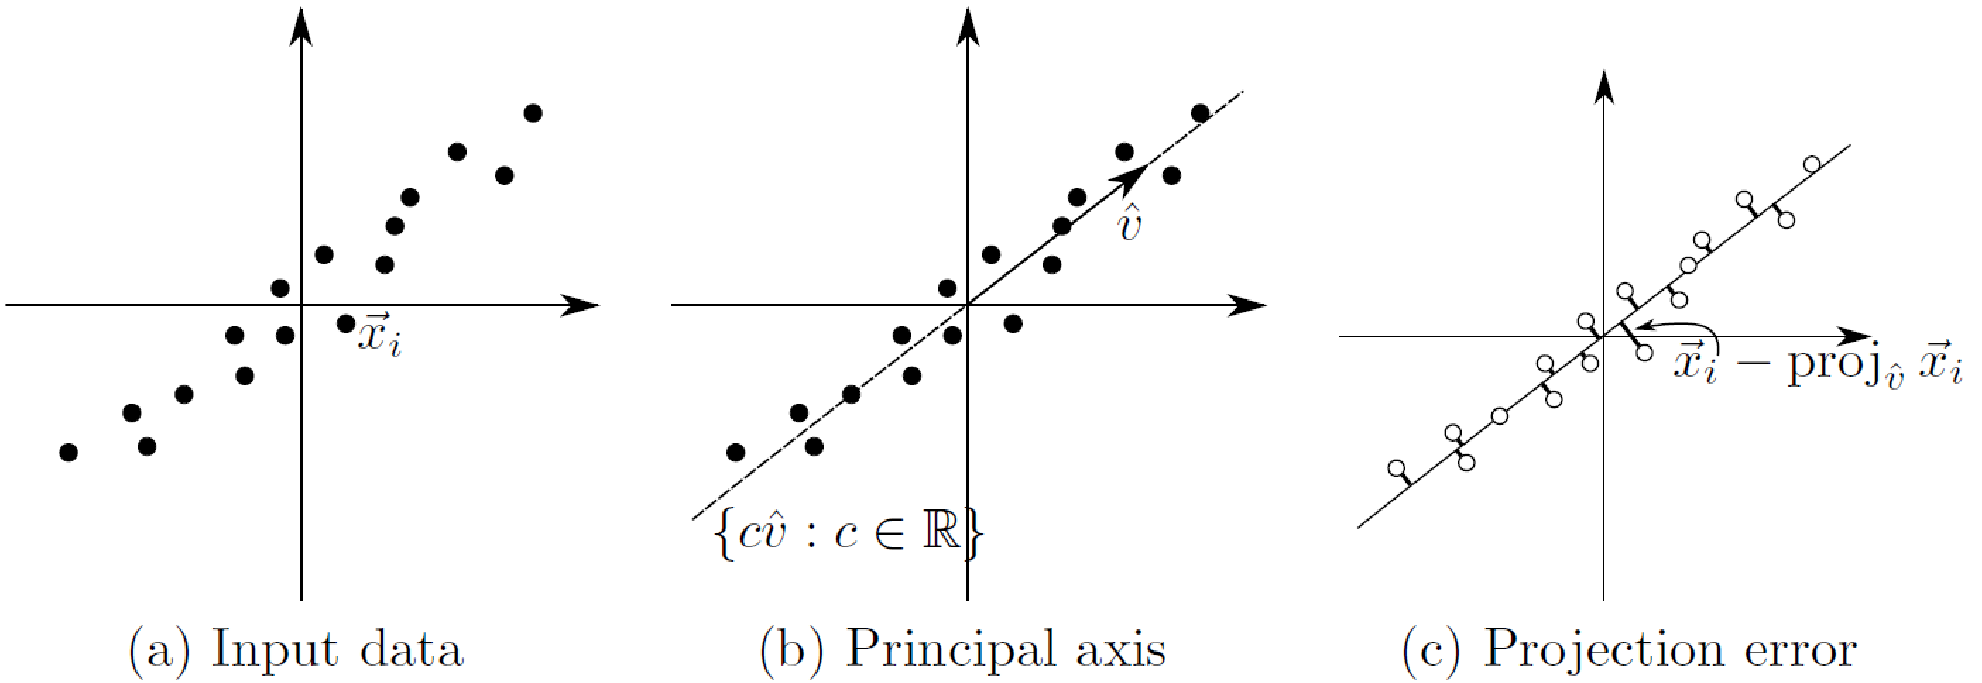
\includegraphics[width=12cm]{principal_axis.png}\end{center}
        Stiamo cercando una retta, in modo analogo a abbiamo visto con la regressione lineare, ma il criterio di 
        minimizzazione è diverso: vogliamo minimizzare la somma di tutte le norme dei complementi ortogonali.
        \[ \min_\mathbf{v} \sum_i \Vert \mathbf{x}_i - \text{proj}_\mathbf{v}\mathbf{x}_i \Vert_2^2 \quad \text{t.c. }\Vert\mathbf{v}\Vert_2 = 1\]
        Il vincolo sulla norma non è necessario, ma semplifica come risolvere il problema di ottimizzazione. Il vettore 
        $\mathbf{v}$ che minimizza l'errore si chiama \emph{asse principale}. 
        Osserviamo che possiamo traslare il problema in notazione matriciale:
        \[ \min_\mathbf{v} \sum_i \Vert \mathbf{x}_i - \text{proj}_\mathbf{v}\mathbf{x}_i \Vert_2^2 \quad \text{t.c. }\Vert\mathbf{v}\Vert_2 = 1\]
        \[ = \min_\mathbf{v} \sum_i \Vert \mathbf{x}_i - \frac{\mathbf{x}_i^T\mathbf{v}}{\mathbf{v}^T\mathbf{v}}\mathbf{v} \Vert_2^2 \quad \text{t.c. }\Vert\mathbf{v}\Vert_2 = 1\]
        Dato che la norma è uguale a 1:
        \[ = \min_\mathbf{v} \sum_i \Vert \mathbf{x}_i - (\mathbf{x}_i^T\mathbf{v}) \mathbf{v} \Vert_2^2 \quad \text{t.c. }\Vert\mathbf{v}\Vert_2 = 1 \]
        Espandiamo la norma al quadrato:
        \[ = \min_\mathbf{v} \sum_i (\mathbf{x}_i - (\mathbf{x}_i^T\mathbf{v}) \mathbf{v})^T(\mathbf{x}_i - (\mathbf{x}_i^T\mathbf{v}) \mathbf{v})  \quad \text{t.c. } \Vert \mathbf{v} \Vert_2 = 1 \]
        Effettuiamo i prodotti e semplici passaggi algebrici:
        \[ = \min_\mathbf{v} \sum_i (\Vert \mathbf{x}_i \Vert_2^2 - 2(\mathbf{x}_i^T \mathbf{v})(\mathbf{x}_i^T\mathbf{v}) + (\mathbf{x}_i^T \mathbf{v})^2 \Vert \mathbf{v} \Vert_2^2)\quad \text{t.c. } \Vert \mathbf{v} \Vert_2 = 1\]
        \[ = \min_\mathbf{v} \sum_i (\Vert \mathbf{x}_i \Vert_2^2 - 2(\mathbf{x}_i^T \mathbf{v})^2 + (\mathbf{x}_i^T \mathbf{v})^2 \Vert \mathbf{v} \Vert_2^2)\quad \text{t.c. } \Vert \mathbf{v} \Vert_2 = 1\]
        \[ = \min_\mathbf{v} \sum_i (\Vert \mathbf{x}_i \Vert_2^2 - (\mathbf{x}_i^T \mathbf{v})^2)\quad \text{t.c. } \Vert \mathbf{v} \Vert_2 = 1\]
        Semplifichiamo eliminando il valore che non dipende da $\mathbf{v}$:
        \[ = \min_\mathbf{v} - \sum_i (\mathbf{x}_i^T\mathbf{v})^2 \quad \text{t.c. } \Vert \mathbf{v} \Vert_2 = 1\]
        Ora sia $\mathbf{X}$ la matrice che contiene i vettori $\mathbf{x}_i$ come colonne:
        \[ = \min_\mathbf{v} - \Vert \mathbf{X}^T \mathbf{v} \Vert_2^2 \quad \text{t.c. } \Vert \mathbf{v} \Vert_2 = 1\]
        \[ = \max_\mathbf{v} \Vert \mathbf{X}^T\mathbf{v} \Vert^2_2 \quad \text{t.c. } \Vert \mathbf{v} \Vert_2 = 1\]
        Che può anche essere riscritto come:
        \[\max_\mathbf{v} \mathbf{v}^T\mathbf{XX}^T\mathbf{v}\quad \text{t.c. } \Vert \mathbf{v} \Vert_2 = 1 \]
        Il massimizzatore che risolve il problema $\mathbf{v^*}$ è il \emph{componente principale} dei dati contenuti 
        nella matrice $\mathbf{X}$.

    \section{Autovettori e autovalori}
        Un autovettore $\mathbf{x}$ di una matrice quadrata $\mathbf{A}$ è un qualsiasi vettore che soddisfa la seguente 
        espressione:
        \[\mathbf{Ax} = \lambda\mathbf{x} \quad \text{per qualche valore }\lambda\text{ anche complesso}\]
        Il valore $\lambda$ è l'\emph{autovalore} dell'autovettore $\mathbf{x}$.
        Intuitivamente, gli autovettori di una mappa lineare $\mathbf{A}$ sono quei vettori che, quando applichiamo $\mathbf{A}$,
        vengono solo scalati del valore $\lambda$, non vengono ruotati.
        \paragraph{La scala di un autovettore non è importante} In particolare:
        \[\mathbf{A}c\mathbf{x} = c\mathbf{Ax} = c \lambda \mathbf{x} = \lambda c\mathbf{x} \]
        Per qualunque $c$, otteniamo sempre lo stesso $\lambda$. Per questa ragione ci limiteremo quindi a cercare gli 
        autovettori di norma 1.
        \paragraph{Similarità di trasformazioni lineari} Consideriamo la seguente trasformazione lineare invertibile:
        \[\mathbf{ATx} = \lambda\mathbf{Tx}\]
        Stiamo dicendo che $\mathbf{Tx}$ è un autovettore di $\mathbf{A}$ con autovalore $\lambda$. Ora proviamo 
        ad applicare la trasformazione lineare $\mathbf{T}^{-1}$ a sinistra:
        \[\mathbf{T}^{-1}\mathbf{ATx} = \lambda \mathbf{x}\]
        Possiamo osservare che $\mathbf{x}$ è un autovettore di $\underbrace{\mathbf{T}^{-1}\mathbf{AT}}_\mathbf{B}$ 
        con autovalore $\lambda$.
        Poiché le trasformazioni lineari $\mathbf{A}$ e $\mathbf{B}$ hanno gli stessi autovalori, 
        diciamo che esse sono \emph{simili} o \emph{co-spettrali} o \emph{iso-spettrali}.
        \paragraph{Autovalori di matrici ortogonali}
        Osserviamo ora una proprietà importante delle matrici ortogonali, esse hanno tutti autovalori $\pm1$:
        \[\mathbf{Qx} = \lambda \mathbf{x}\]
        \[= \Vert\mathbf{Qx}\Vert_2^2 = \Vert \lambda \mathbf{x} \Vert_2^2 \]
        \[ = (\mathbf{Qx})^T\mathbf{Qx} = |\lambda|^2\Vert \mathbf{x}\Vert_2^2\]
        \[ = \mathbf{x}^T\mathbf{Q}^T\mathbf{Qx} =|\lambda|^2\Vert \mathbf{x}\Vert_2^2 \]
        \[ = \mathbf{x}^T\mathbf{x} = |\lambda|^2\Vert\mathbf{x}\Vert_2^2\]
        \[ = \Vert\mathbf{x}\Vert_2^2 = |\lambda|^2\Vert\mathbf{x}\Vert_2^2\]
        \[ = 1 = |\lambda|^2\]
        \[ \lambda = \pm 1\]
        \paragraph{Autovalori di matrici diagonali o triangolari superiori}
        Gli autovalori di tali matrici sono i valori sulla diagonale principale.
        \paragraph{Autovalori di matrici simmetriche}
        Ricordiamo che una matrice $\mathbf{A}$ è simmetrica se $\mathbf{A} = \mathbf{A}^T$. \\
        Possiamo affermare che tutti gli autovalori di una matrice simmetrica sono reali. Consideriamo la coppia
        autovalore-autovettore $(\lambda, \mathbf{x})$ tale che $\Vert \mathbf{x} \Vert_2^2=1$:

        \begin{align*}
            \lambda \mathbf{x}^T\mathbf{x} &= (\lambda \mathbf{x})^T\mathbf{x} \\
            &=(\mathbf{Ax})^T\mathbf{x}\\
            &=\mathbf{x}^T\mathbf{A}^T\mathbf{x} \\
            &=\mathbf{x}^T(\mathbf{Ax}) \\
            &=\overline{(\mathbf{Ax})^T\mathbf{x}} \quad \text{in cui $\overline{z}$ è il coniugato di $z$}\\
            &=\overline{(\lambda\mathbf{x})^T\mathbf{x}} \\
            &=\overline{\lambda}\mathbf{x}^T\mathbf{x}
        \end{align*}
        Consideriamo ora due distinti autovettori $\mathbf{x}_i,\mathbf{x}_j$ con $\lambda_i \neq \lambda_j$:
        \[(\mathbf{Ax}_i)^T\mathbf{x}_j = \mathbf{x}_i^T\mathbf{Ax}_j\]
        \[(\lambda_i \mathbf{x_i})^T \mathbf{x}_j = \mathbf{x}_i^T\lambda_j\mathbf{x}_j\]
        Questo significa che $\mathbf{x}_i^T\mathbf{x}_j = 0$, ovvero $\mathbf{x}_i$ e $\mathbf{x}_j$ sono ortogonali.
    
        \paragraph{Autovettori di matrici che commutano}
        Consideriamo due matrici $\mathbf{A}$ e $\mathbf{B}$. Possiamo dire che:
        \[\mathbf{AB} = \mathbf{BA} \Leftrightarrow \mathbf{A} \text{ e }\mathbf{B} \text{ hanno gli stessi autovettori}\] 
        Possiamo anche osservare che non è detto che $\mathbf{A}$ e $\mathbf{B}$ abbiano gli stessi autovalori:
        \[\mathbf{v}^T\mathbf{Av} = \lambda \neq \mu = \mathbf{v}^T\mathbf{Bv}\]
        \paragraph{Teorema di Courat}
            L'autovettore associato all'autovalore massimo si chiama \emph{autovettore principale}.

    \section{Asse principale \small{(continua)}}
        Torniamo al nostro problema: dobbiamo fittare una retta tra dei punti minimizzando l'errore quadratico medio 
        perpendicolare alla retta:
        \begin{center}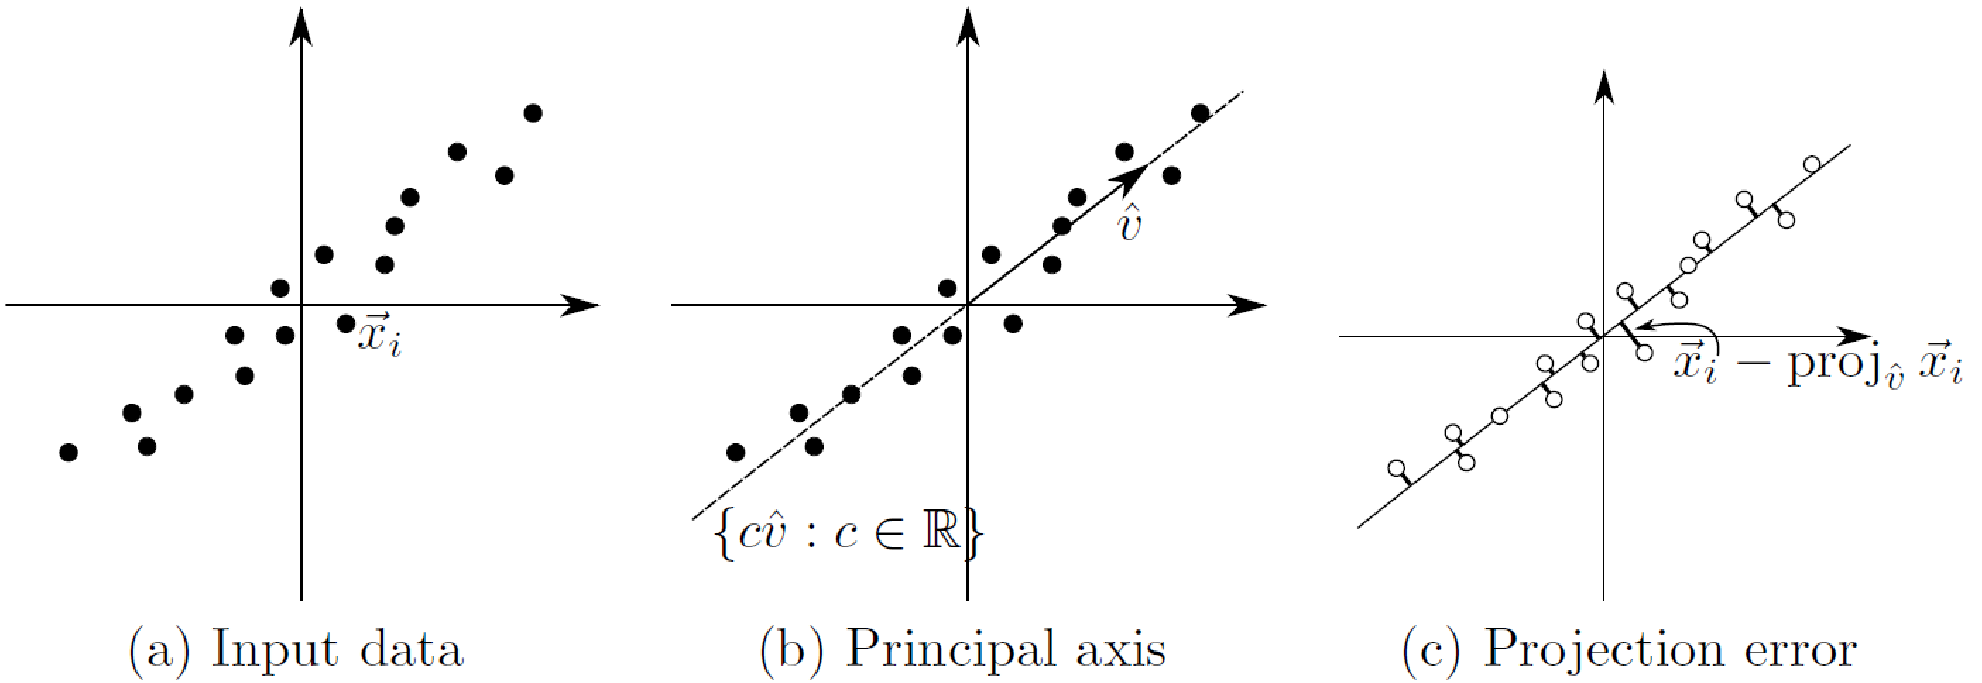
\includegraphics[width=12cm]{principal_axis.png}\end{center}
        Per risolvere il problema dobbiamo trovare il vettore $\mathbf{v}$.
        \[\max_{\mathbf{v}} \mathbf{v}^T \underbrace{\mathbf{XX}^T}_\text{simmetrica} \mathbf{v}\]
        \subsection{Teorema min-max}
            Se $\mathbf{A}$ è una matrice simmetrica, allora il suo autovalore massimo è dato dalla seguente equazione:
            \[\max_\mathbf{v} \frac{\mathbf{v}^T\mathbf{Av}}{\Vert \mathbf{v} \Vert_2^2}\]
            con $\mathbf{v}$ il corrispettivo autovettore. Più in generale:
            \[\lambda_{\text{min}} \leq \frac{\mathbf{v}^T\mathbf{Av}}{\Vert \mathbf{v} \Vert_2^2} \leq \lambda_{\text{max}}\]
            In cui il quoziente $\frac{\mathbf{v}^T\mathbf{Av}}{\Vert \mathbf{v} \Vert_2^2}$ è chiamato \emph{quoziente di Rayleigh}.

    \section{Teorema spettrale}
        L'insieme di autovalori $\{\lambda_i\}$ di una matrice $\mathbf{A}$ è chiamata \emph{spettro}. Possiamo scrivere 
        l'equazione degli autovalori come:
        \[\mathbf{AX} = \mathbf{X\Lambda} \]
        Se $\mathbf{A}$ è simmetrica, allora $\mathbf{X}$ è una matrice ortogonale di autovettori e $\mathbf{\Lambda}$ è la matrice
        diagonale con autovalori reali. L'equazione appena mostrata possiamo scriverla anche nel seguente modo:
        \[\mathbf{X}^T \mathbf{AX} = \mathbf{\Lambda} \]
        E tale equazione è chiamata la \emph{decomposizione spettrale} di $\mathbf{A}$. Osserviamo che essa è molto simile al problema 
        dell'asse principale:
        \[\max_{\mathbf{x}} \mathbf{x}^T\mathbf{Ax} \quad \text{t.c. }\Vert\mathbf{x}\Vert_2 = 1 \quad \text{asse principale}\]
        Modifichiamo il problema per risolvere per tutti gli autovettori e i rispettivi autovalori:
        \[\min_{\mathbf{X}} \text{tr}(\mathbf{X}^T\mathbf{AX}) \quad \text{t.c. }\mathbf{X}^T\mathbf{X}=\mathbf{I} \quad \text{decomposizione spettrale}\]
        In questo problema stiamo minimizzando con il vincolo che $\mathbf{X}$ sia ortogonale. Tale quesito non è convesso, 
        ovvero non è banale trovare 
        una soluzione globale al problema ma, per questo in problema in particolare, esistono algoritmi che permettono di risolverlo globalmente. 
\newpage
    \section{Trovare gli autovalori}
        \paragraph{Autovettore massimo (power iteration)}
        Un algoritmo molto semplice per trovare l'autovalore più grande è quello della \emph{normalized-iteration}, 
        mostrato in seguito:
        \begin{algorithm}
            \caption{Normalized-Iteration}
            \label{Normalized-Iteration}
            \begin{algorithmic} % The number tells where the line numbering should start
                \Function{Normalized-Iteration}{$A$}
                    \State $\vec{v} \gets \text{Arbitrary}(n)$
                    \For{$k \gets 1, 2, 3, \dots$}
                        \State $\vec{w} \gets A\vec{v}$ 
                        \State $\vec{v} \gets {\vec{w}}/\Vert{\vec{w}}\Vert$ \Comment la normalizzazione è atta a ridurre errori numerici
                    \EndFor
                    \State \Return $\vec{v}$
                \EndFunction
            \end{algorithmic}
        \end{algorithm}

        \paragraph{Autovalore minimo (inverse iteration)}
            Per trovare l'autovettore minimo osserviamo che:
            \[\mathbf{Ax} = \lambda\mathbf{x} \Rightarrow \mathbf{A}^{-1}\mathbf{x} = \frac{1}{\lambda}\mathbf{x}\]
            Da ciò ne concludiamo che possiamo semplicemente applicare il power method a $\mathbf{A}^{-1}$. Tuttavia, esistono 
            tecniche più efficienti che non prevedono l'inversa di $\mathbf{A}$, come la decomposizione LU.

        \subsection{Iterazione QR}
            Abbiamo già visto nella sezione 2. che se $\mathbf{B} = \mathbf{T}^{-1}\mathbf{AT}$, allora $\mathbf{A}$ e 
            $\mathbf{B}$ hanno lo stesso spettro, ovvero sono matrici simili. Per cui potremmo prima ottenere una decomposizione 
            $\mathbf{QR}$ di $\mathbf{A}$:
            \[\mathbf{A} = \mathbf{QR}\]
            E poi sovrascrivere $\mathbf{A}$, mantenendo ancora gli stessi autovalori:
            \[\mathbf{A} \gets \mathbf{Q}^T\mathbf{AQ}\]
            Ora osserviamo:
            \[\mathbf{Q}^T\mathbf{AQ} = \mathbf{Q}^T(\mathbf{QR})\mathbf{Q} = (\mathbf{Q}^T\mathbf{Q})\mathbf{RQ} = \mathbf{RQ}\]
            In altre parole, questa operazione preserva gli autovalori:
            \[\mathbf{A} \gets \mathbf{RQ}\]
            Se continuiamo ad effettuare questa operazione in modo iterativo, otteniamo l'algoritmo \emph{QR-Iteration}: 
\newpage
            \begin{algorithm}
                \caption{QR-Iteration}
                \label{QR-Iteration}
                \begin{algorithmic} % The number tells where the line numbering should start
                    \Function{QR-Iteration}{$A \in \mathbb{R}^{n \times n}$}
                        \For{$k \gets 1, 2, 3, \dots$}
                            \State $Q,R \gets \text{Fattorizzazione-QR(A)}$ 
                            \State $A \gets RQ$
                        \EndFor
                        \State \Return $\text{diag}({R})$
                    \EndFunction
                \end{algorithmic}
            \end{algorithm}
            Facciamo alcune osservazioni:
            \begin{enumerate}
                \item Tutte le matrici intermedie generate dall'algoritmo $\mathbf{A}_1, \mathbf{A}_2, \dots$ hanno gli stessi autovalori
                \item Le iterazioni convergono, ovvero a un certo punto $\mathbf{A}_k \approx \mathbf{A}_{k-1}$
                \item A convergenza, otteniamo $\mathbf{Q}_\infty^T\mathbf{A}_\infty\mathbf{Q}_\infty = \mathbf{A}_\infty$, il che implica \\
                $\mathbf{Q}_{\infty}\mathbf{R}_\infty = \mathbf{R}_\infty \mathbf{Q}_\infty$ e $\mathbf{A}_\infty \mathbf{Q}_\infty = \mathbf{Q}_\infty \mathbf{A}_\infty$
                \item Se $\mathbf{A}_\infty \mathbf{x} = \lambda\mathbf{x}$ allora possiamo scrivere:
                    \[\lambda \mathbf{x} = \mathbf{A}_\infty\mathbf{x} = \mathbf{Q}_\infty \mathbf{R}_\infty \mathbf{x} = \mathbf{R}_\infty \mathbf{Q}_\infty \mathbf{x} = \pm\mathbf{R}_\infty \mathbf{x}\]
                    L'ultima parte dell'uguaglianza deriva dal fatto che gli autovalori di $\mathbf{Q}$ sono $\pm1$ poiché essa è ortogonale. 
                    In altre parole, gli autovalori di $\mathbf{A}_\infty$, e quindi anche quelli di $\mathbf{A}$, sono uguali agli elementi 
                    sulla diagonale di $\mathbf{R}_\infty$ a parte il segno. 
            \end{enumerate}
            
    \section{Shifting}
        Data una matrice $\mathbf{A}$ con autovalori $\{\lambda_i\}$ e autovettori $\{\mathbf{x}_i\}$:
        \[( \mathbf{A} - \sigma\mathbf{I})\mathbf{x}_i = \mathbf{Ax}_i - \sigma\mathbf{x}_i = \lambda_{\mathbf{x}_i} - \sigma\mathbf{x}_i = (\lambda_i - \sigma)\mathbf{x}_i\]
        Che significa che gli autovalori di $\mathbf{A} - \sigma\mathbf{I}$ sono $\lambda_i - \sigma$, ovvero effettuando 
        uno shift sulla matrice otteniamo lo stesso shift anche sui suoi autovalori. \\
        Possiamo osservare che se $\sigma$ è vicino all'autovalore di $\mathbf{A}$, allora $\mathbf{A} - \sigma\mathbf{I}$ ha 
        un autovalore vicino allo 0. Possiamo usare questo fatto per stimare porzioni dello spettro di $\mathbf{A}$:
        \begin{enumerate}
            \item Effettuiamo un ipotesi su un autovalore
            \item Computiamo la matrice shiftata $\mathbf{B} = \mathbf{A} - \sigma\mathbf{I}$
            \item Applichiamo l'inverse iteration su $\mathbf{B}$ per trovare l'autovalore minimo. 
        \end{enumerate}

\end{document}